% -*- mode:LaTex; mode:visual-line; mode:flyspell; fill-column:75-*-

\chapter{Backgound \& Related Work} \label{chapBackground}
\section{Informing Forest Management}
%\begin{itemize}
%    \item Fuel classification
%    \item Species classification
%    \item Health/alive/dead
%    \item Biomass regression
%    \item Height/DBH estimation
    
Forests worldwide are increasingly under human management. People make decisions for a variety of reasons, ranging from timber growth, wildlife conservation, forest fire mitigation, and carbon sequestration. These decisions should be informed by the current state of the forest. Examples include the type of dominant vegetation at a given location, or the location, height, diameter, health, or species of individual trees.

In practice, management decisions are only made with limited imperfect estimates of these quantities. A common approach is that foresters conduct manual laborious surveys of a set of small hand-chosen plots and extrapolate these measurements to the unobserved regions. This is an extremely time-consuming process and is heavily reliant on choosing representative survey sites and using domain knowledge to accurately extrapolate to unseen regions.
Despite the limitations, this data often represents the richest and most detailed understanding of a region.

Another approach for understanding forests using remote sensing data captured from satellites or crewed aircraft.

\begin{itemize}
    \item Talk more about the two applications we're considering, fire management and carbon sequestration
    \item 
\end{itemize}

\subsection{Manual forestry cruises}
\begin{itemize}
    \item Describe how this is currently done
    \item Find a reference for the pain points
\end{itemize}

\subsection{Using satellites and crewed aircraft for forest management}
\begin{itemize}
    \item talk about what what sat is 
    \item Sat data has a broad extent and may be too low res
    \item Reannalysis has shown that accuracy is often very low \cite{} 
    \item Data products from crewed aircraft has higher resolution but require substaintial investment and planning
\end{itemize}

\subsection{Drone surveys in forestry}
\begin{itemize}
    \item Describe a bit about what drones are  
    \item OFO work \cite{Young2022} 
\end{itemize}

\section{Automated methods for understanding forest structure}
\subsection{Photogrametry}
In general, commodity drones produce only monocular images with potentially a low-accuracy GPS and orientation estimate. A common approach for estimating geometric from this type of data is photogrametry, also known as structure from motion or 3D reconstruction. The origins of photogrametry date back to WWII where it was a manual processed to estimate the geometry of structures from aerial images. Modern automated approaches began todo. Preliminary reconstructions of realistic large-scale scenes began with academic work such as \cite{Agarwal2009}. Over the last decade, numerous commercial and open-source software have been developed to accomplish the task. Some examples include: Agisoft Metashape, COLMAP, OpenMVG, OpenDroneMap.

The details vary by application and assumption, but a common pipline is the following. First, distinctive features are detected in each image. These represent small patches of pixels which are likely to be distinctive, such as corners and edges. Then, features are matched between images, based on the local appearance. 
Given these correspondences, multiple things can be estiated. The first is the location of these matched points in the 3D space, using triangulation between the cameras. The second is the location of the cameras. Finally, if the camera isn't accurately calibrated, it's common to estimate the parameters which describe how points in the world appear on the image. Given the interplay between all of these elements, it's critical to estimated them together in a global joint optimization. The class of techniques for solving this problem are termed bundle adjustment and are often build on iterative nonlinear least squeres. 

After these quantities are estimated, it's common to re-estimate the correspondences between images using the existing solution as a way to filter incorrect correspondes which are not consisent with the majority of other matches. These steps are often the focus of extensive engineering effort to improve the final performance. 

After this iterative process converges, the result is a sparse output consisting of the camera locations and calibration parameters as well as a sparse set of 3D locations. This sparse representation doesn't capture the full geometry of the scene, since only the most distinctive points are represented. Moreover, because it is a pointcloud, we cannot reason about which parts of the scene would obstuct or "occlude" the view of another one. To accomplish these tasks, we leverage the fact that many solvers can produce a mesh representation of the surface of the scene. A mesh is a common representation in computer vision and graphics, which consists of a set of 3D points connected by triangular faces. 

The process of mesh computation varies by solver. A common first step is to estimate the likely depth to the surface from each camera using color constancy. This means that for a set of posible distances, the observed color from that camera is checked against the color which would be observed by the other camera, if that were the true location of the surface. From this information, a predicted most likely depth surface is predicted for each pixel. Then, the predicted depth is combined across all cameras to produce a consistent 3D geometry. This is often done using a truncated signed distance function representation \cite{} 

\begin{figure}
    \centering
    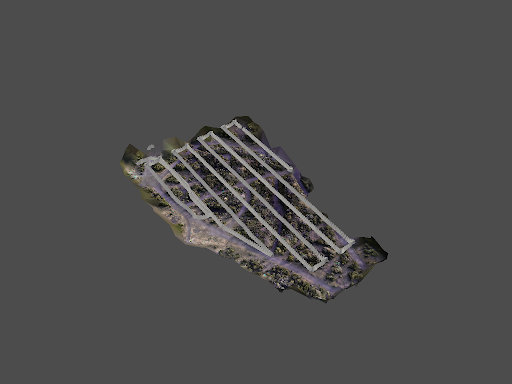
\includegraphics[width=\textwidth]{figs/methods/structure_from_motion/camera estimation.png}
    \caption{The estimated camera locations in space}
    \label{fig:camera-locations}
\end{figure}

These solvers are becoming increasingly robust, and are well-suited to reconstructing scenes captured by drone surveys because the same location is often seen across many images.

\subsection{SLAM}
Structure from motion is a powerful tool, but a key limitation is that it can only be used to map the environment after a mission is complete. In settings where a drone is operating autonomously in complex environment such as under the canopy, it is important that it understands where it is in relation to obstacles in real time. This problem is challenging because it requires completing two challenging tasks at once: building a map of the world while estimating where the robot is within the map. This problem is known in the robotics literature as simultaneous localization and mapping (SLAM). This refers to the fact that in a new environment, the robot must build a map of the world at the same time as figuring out where it is in this map. 


\section{Automated methods for understanding attributes of forests}
\subsection{Semantic segmentation}
\begin{itemize}
    \item Talk about what semantic segementation is
    \item Cite early work such as FCN and U-Net
    \item Talk about largescale benchmarks such as CityScapes and explain why those aren't as applicable as we'd hope for our domains.
    \item Cite Segformer \cite{Xie2021}, SegNext \cite{Guo2022SegNeXt:Segmentation} and try to describe the concepts behind transformer-based architectures
\end{itemize}
\subsection{Semantic mapping}

\begin{itemize}
    \item Talk about what we mean by semantic mapping 
    \item Talk about some generic approaches: UFO map \cite{Duberg2020UFOMap:Unknown}, Kimera \cite{Rosinol2020}
    \item Our semantic mapping \cite{RussellUnmannedMitigation} that was derived from \cite{semantic_slam_RGBD}
    \item Talk about land-use mapping approaches from ecologists \cite{Liu2018DeepClassification} 
\end{itemize}


To the best of our knowledge, one of the first works that explores semantic mapping in a forestry context is \cite{Andrada2022IntegrationRoboticsb}. This focuses on a multi-sensor ground vehicle.

\section{Detecting trees in top-down imagery}
We chose to use DeepForest \cite{Weinstein2020DeepForest:Delineation} in this work because it's a commonly-used approach that was trained on a diverse set of trees from the national ecological observation network (NEON) \cite{Keller2008ANetwork} across the country.

Talk about DetectTree2 \cite{DetectTree2} \\
Talk about CHM approaches
Go through Derek's paper and find other ones.

\section{Planning informative drone surveys}

In many forestry applications, the region of interest is commonly substantially larger than what is feasible to survey, either by hand or even with a drone. In practice, foresters  select a small set of plots to visit and extrapolate from these sparse observations to the entire region. These plots are chosen using expert knowledge of the region to be diverse and representative.

Despite the ability of drones to cover much large regions than humans alone, they still fall short of the ability to perform  exhaustive coverage. For example, rough calculations suggest that it would take a drone pilot 250 full days flying to survey the TODO region. Therefore, it is clear that judicious use of limited resources is critical.

Satellite or aerial data is the primary modality of data that scales to the extent required for understanding forests at scale. Unfortunately, prior work has shown that many existing satellite prediction models are highly inaccurate \cite{}. Furthermore, useful global models exist only for select satellite data product and for common tasks like biomass estimation. Therefore, they are not applicable when improved satellites are launched or if a regional satellite or aerial campaign is conducted.
It is possible to tackle fine-grained tasks such as species classification with satellite data, but they are often only relevant to a small region \cite{Sweden}. 
Therefore, we wish to streamline the process of developing satellite prediction models by using a generic framework and fitting it to local observations.

Specifically, we assume that our drone collects data that can be accurately interpreted to predict the quantity of interest. For example, we can task a human annotator with identifying tree species from high-resolution drone images, or train a deep learning model to do the same. We further assume that information relavent to this task is contained in remote sensing data of the scene, but it's not easy or scalable to label this data directly. This may be because a human labeller does not possess the intuition to label species based solely on low-resolution satellite data. This claim is especially relevant if the remote sensing data contains channels other than Red-Green-Blue, as it is hard for humans to fully interpret this data \cite{Hard to label multispectral}.

Given these assumptions, the goal is to choose a set of sample locations to observe with the drone. From these observations, we obtain a classification label for each observed pixel in the remote sensing data. We then train a satellite prediction system using these observed pixels as the ground truth training examples. The goal of this work is to observe regions which serve as useful training samples for this satellite prediction system. This is similar to the ideas of active learning \cite{Active learning}, where a repository of unlabeled data is available and an algorithm can query an oracle for labels of a subset of samples. However, active learning is not directly applicable to our domain since in classical formulations, any combination of samples can be selected. In this work, the samples relate to spatial regions that must be visited by a drone. Therefore, it must be possible to visit all the requested samples subject to operational constraints such as the drone's battery life.

This problem is most closely related to prior work in informative path planning (IPP). This diverse field is concerned with how and were to sample observations with an agent to gain some understanding of a phenomena of interest. Due to the diversity of application domains which have their own specific objectives, assumptions, and constraints, there are a diversity of approaches tackling this broad problem. For our domain, a desirable informative path planning algorithm:

\begin{itemize}
    \item \textbf{Considers non-spatial features:} Since we assume that we have prior satellite or low-resolution aerial data of a scene, it is important that an intelligent algorithm leverages this information.
    \item \textbf{Plans over a long horizon:} The commodity drones considered in this work must execute a plan developed prior to launch, e.g. offline, and cannot replan in-flight.
    Therefore, it is important that the algorithm can produce a plan which can be executed for many observations sequentially, ideally as many as can be taken before the battery must be replaced. 
    \item \textbf{Is computationally fast and scalable:} We desire that this algorithm can be executed on a laptop in the field to enable easy deployment.
    To be operationally useful, it must be possible to develop a plan for a new---potentially large---region in a short period of time.
    \item \textbf{Considers area measurements:} Many informative path planning algorithms assume that an observation is a single point in space. Instead, we want to plan were to observe with a downward-facing camera or where to survey a small region. In either case, these observations cover a region that is too large to be approximated as a single point.
\end{itemize}



Significant work has been done under the assumption that the agent can re-plan its trajectory online, based on the observations it sees during execution. This requires a sophisticated robotic platform that can sense its environment, process this data into a useful format, re-plan which regions would be useful to explore, and execute this plan. In most cases, the agent maintains some sort of belief of which regions uncertain, desirable, or combination of both. At each re-planning iteration, the agent seeks to develop a plan that is likely to optimize its objectives within the operational constraints such as path length.

The work of \cite{Popovic2020} proposes a generic framework for terrain monitoring with UAVs equipped with a downward facing camera. This work assumes that the quantity of interest is a scalar field defined over the environment that has spatial correlations, e.g. similar locations will have similar values. The example use-case is modeling the density of weeds in an agricultural application, where it is most important to accurately model regions with a high infestation. Further, it assumes that the UAV is able to re-plan its trajectory in flight, after taking uncertain measurements of the environment. A strength of this work is that it models the altitude-dependent effects of a drone camera: at higher altitudes the camera can observe more area but the quality of the measurements will be lower. Using an optimization-based framework and a probabilistic sensor model, the algorithm plans a sequence of observations that decrease the uncertainty while focusing on regions of high predicted weed density. This first part of this path is followed until a new plan based on new observations is developed. This approach is shown to be more effective than a uniform coverage plan at a fixed altitude because it can predict which regions will have more weeds and spend more of the sensing budget there. An extension of this work \cite{Stache2021AdaptiveSegmentation} further explores these concepts with real data. Specifically, they use semantic segmentation to identify weeds in the images and fit empirical models to the segmentation accuracy at different altitudes. This work also shows higher accuracy than a non-adaptive baseline. In both cases, a fundamental strength of the approach is the reason we cannot use it in our domain---online re-planning based on the observed data is critical to the performance increase over the baseline.

A key feature of the previous work is that it seeks to model only regions that were observed with the drone. The main decision is how many times to re-observe a region and at what altitude. In our setting, we wish to make observations with a drone and extrapolate beyond them with satellite data. This goal is somewhat related to that of \cite{Ruckin2022}, which seeks to plan a drone flight that collects images to train a deep learning model for land use classification. In this setting, it is assumed that the drone has a downward facing camera that observes a scene. It also possesses a deep learning model that predicts the land use for each pixel, as well as a measure of uncertainty about the prediction. The goal is to collect images, that when labeled by a human annotator after the mission, can be used to update the model the deep learning model so its performance is better on new data. The authors show that collecting images that the current model is uncertain about leads to better performance after retraining. Therefore, when the drone is collecting data, it should prioritize images that the current model is uncertain about. As the drone explores a region, it generates the uncertainty predictions for each observed images, but cannot access the true label. Then, it continuously updates plan that tries to observe new uncertain images, by assuming that unobserved images next to uncertain observed images will also be uncertain. As with the prior work, this approach requires online reasoning to be effective. Furthermore, this approach has a subtly different goal from ours: their goal is to collect images that can be used to train a good model for new drone observations whereas our approach assumes a model exists already for drone data and these predictions can be used to inform a satellite model. 

Some prior work formulates the problem in similar way to our objective. Work by Kodule et. al. \cite{Kodgule2019Non-myopicMeasurements} and an extension by Candela et. al. \cite{Candela2020PlanetaryMapping} explore the problem of where to gather information with a planetary robot, e.g. Mars Rover, given that the whole region has already been observed by a low-fidelity orbiting satellite. Specifically, it is assumed that the world is represented as a grid of pixels each containing a multispectral (8-channel) observation. Then, multiple Gaussian Processes \cite{Rasmussen2004} are defined which uses the spectral values at each pixel as well as the spatial location of each pixel as features. The goal of 

%Due to the assumption of prior imagery, we may leverage approaches from \cite{Candela2021}, which uses an MCTS planner to explore a world for which prior satellite data exists. This work uses a Gaussian Process to model a quantity of interest. It is challenging to directly apply this work because it assumes that each pixel can be regressed individually by the Gaussian Process. This assumption is unlikely to be correct for high spatial and low spectral resolution data since texture within a local neighborhood will likely need to be considered.

%that can be used to gather information to train a good model for satellite data
%Alberto's Planetary , Alberto's Coral \cite{Candela2021}
%Yogi's Coral \cite{Jamieson2020ActiveEnvironments},


\subsection{Offline/batch methods}
\begin{itemize}
    \item \textbf{Ergodic} Ananya's sparse sensing \cite{Rao}
    \item \textbf{Generic} Sankalp's \cite{Arora2017RandomizedConstraints}, Daniela Rus' Correlated orienteering \cite{Yu2016CorrelatedTasks}
    \item \textbf{TIGRIS} \cite{Moon2022TIGRIS:Planning}
    In this work the authors use a sampling based approach. The chance of taking a sample is biased toward those locations which have higher information content. Importantly, this work takes into account the s
\end{itemize}

Ergodic planning, specifically sparse-sensing ergodic planning \cite{Rao}, provides a framework to plan samples over an \textit{information map} which describes how likely each sample is to be valuable. We could derive this information map from the current model prediction in multiple ways. For example, we could specify that samples predicted as rare classes or extreme AGB values are more interesting. Or we could estimate model uncertainty using ensembles or monte-carlo dropout. However, this approach only considers a per-sample interestingness and spatial diversity of samples. In this case, diversity of appearance may matter more than diversity of location. 



\begin{table}[]
\resizebox{\columnwidth}{!}{%
\begin{tabular}{|l|l|l|l|l|l|}
\hline
 & \makecell{Sparse \\ Ergodic \\ Sensing \cite{Rabbi2020Small-ObjectNetwork}} & \makecell{Optimization-\\based \\ replanning \cite{Popovic2017OnlineUAVs}} & TIGRIS \cite{Moon2022TIGRIS:Planning} & \makecell{MCTS on \\ GPs \cite{Candela2020PlanetaryMapping}} & Proposed \\ \hline
\makecell{Non-spatial \\ features} & X & X & X & Y & Y \\ \hline
\makecell{Long horizon} & Y & X & Y & Y & Y \\ \hline
\makecell{Fast \& scalable} & Y & Y & Y & X & Y \\ \hline
\makecell{Area \\ measurements} & X & Y & Y & Y & Y \\ \hline
%\makecell{Incorporates \\ non-trivial \\ dynamics} & Y & Y & Y & N & N \\ \hline
\end{tabular}%
}
\caption{A comparison of the capabilities of existing informative path planning algorithms.}
\label{tab:my-table}
\end{table}

We can apply concepts from online approaches to offline approaches
We can close the gap between online and offline approaches 

